\section{Experimental Result}
The prilimanary result

\subsection{Best Match}
As we have got the clustering result, a best match method given below is
deployed to evaluate the precision of the split.

\begin{algorithm}[H]
\caption{Best match evaluation algorithm}
\label{best_match}
\begin{algorithmic}[1]
\REQUIRE{$n$ clusters of programs as the result $R$, $m$ sets of programs watched by the m people as the ground truth $T$}
\ENSURE{The best match precision of the split}
\IF{$n \geq m$}
        \STATE $T \Leftarrow T$ add $(n-m)$ empty sets
\ELSE
        \STATE $R \Leftarrow R$ add $(m-n)$ empty sets
\ENDIF
\STATE $precision \leftarrow 0$
\FORALL{bijection $f$ from $R$ to $T$}
        \STATE $cnt \leftarrow 0$
        \FORALL{cluster $r$ in $R$}
                \STATE $cnt \leftarrow cnt + numberOfIntersections(r, f(r))$
        \ENDFOR
        \IF{$match > precision$}
                \STATE $precision \leftarrow match$
        \ENDIF
\ENDFOR
\RETURN $precision$
\end{algorithmic}
\end{algorithm}

Under such evaluation, the precision is 100\% when everything gets right. If we do not predict the
number of users correctly (more or less users are detected), we will be charged with a heavy penalty
that some empty sets are involved such that no result will match on them, which has a large impact on
the result.

For instance, given a sequence watched by 3 different people who respectively watched \{A, B\}, \{C, D\}, \{E, F, G\} programs,
if our algorithm predicts it is watched by 2 people with the clusters \{A, B, C\} and \{D, E, F, G\}, the precision will be
71.4\% where A, B, E, F, G are matched in the best match.

\subsection{Experiment Setup}
We tested our approach and baseline method in 16 viewing sequences. The 16 viewing sequences consist of 4 groups with 4 sequences in each group.
The group is divided by the number of viewer behind the sequence. The distribution of this 16 viewing sequences is depicted in figure \ref{fig:distribution}.

\begin{figure}[htbp]
\centering
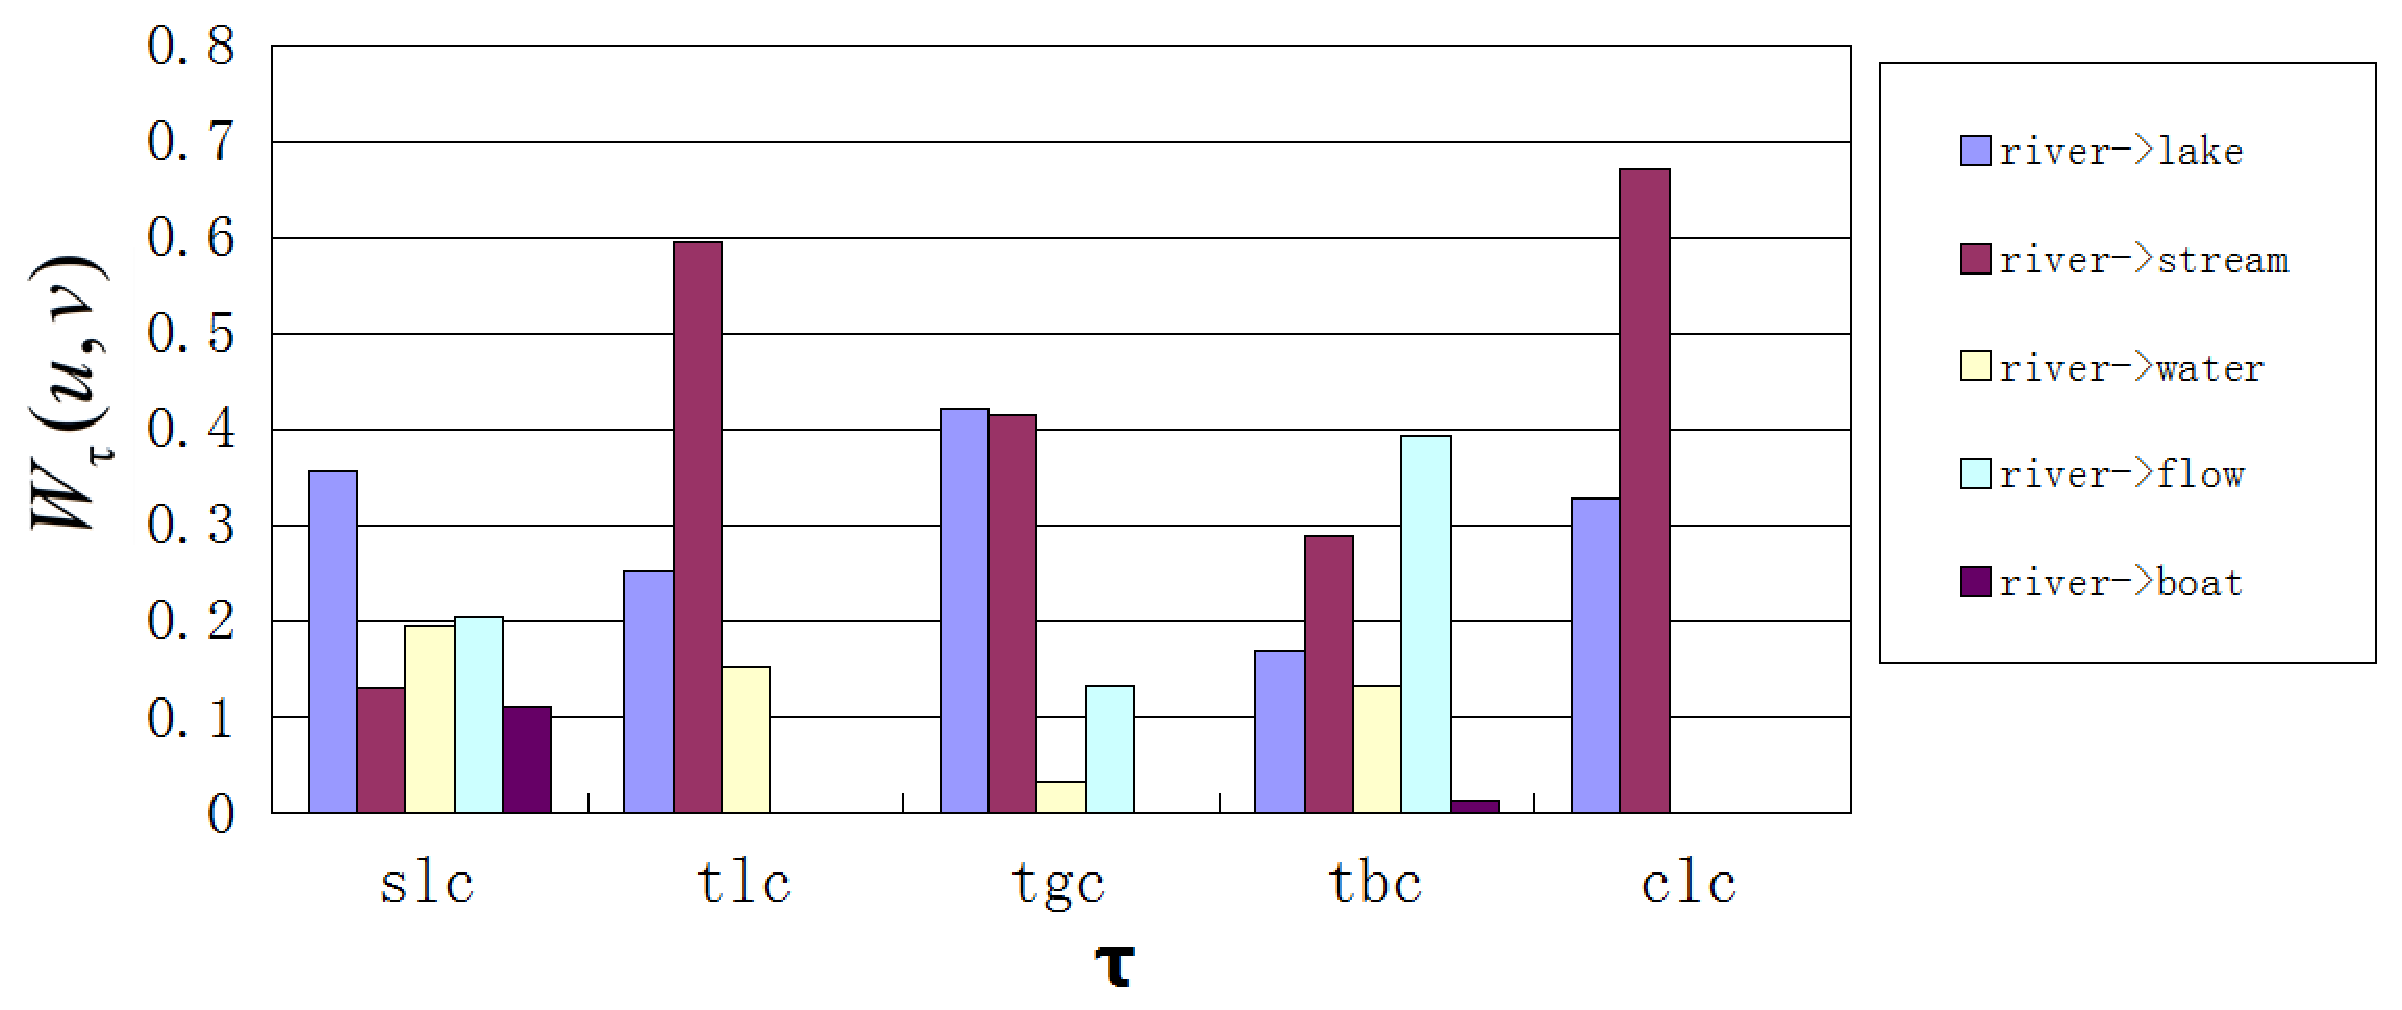
\includegraphics[width=3.0in]{distribution.eps}
\caption{Test Sequences Illustration}
\label{fig:distribution}
\end{figure}

We test our approach for each of the test sequence.

\subsection{Experiment Result}
\subsubsection{Precision of Splitting the Watching Sequence}
In figure \ref{fig:exresult}, we list the comparison results of our approach and baseline approach. The comparison is from different perspective.
Figure \ref{fig:point-wise} shows that for the majority of the test sequence our approach over-performs the base-line approach. Figure \ref{fig:group-wise}
shows that for different group size our approach over-performs the base-line approach.

\begin{figure*}
\subfigure[Precision Comparision by each point]{\label{fig:point-wise}\includegraphics[width=0.66\columnwidth]{point-compare.eps}}
\subfigure[Precision Comparision by group size]{\label{fig:group-wise}\includegraphics[width=0.66\columnwidth]{compare.eps}}
\subfigure[Overall Presicion Comparison]{\label{fig:over}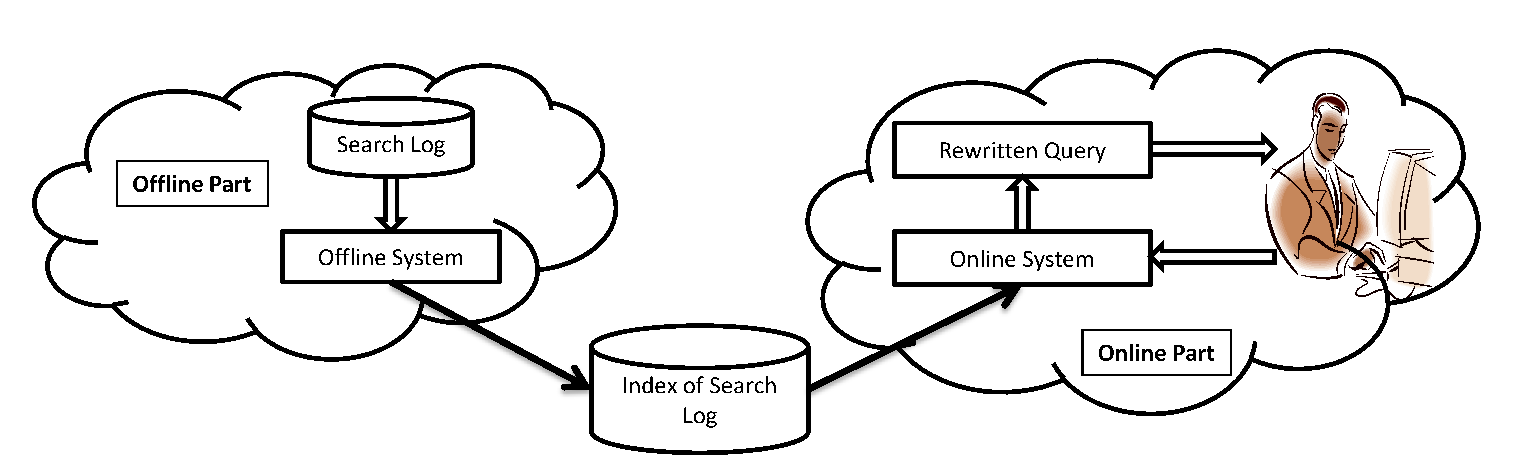
\includegraphics[width=0.66\columnwidth]{overall.eps}}
\caption{Experimental Result}
\label{fig:exresult}
\end{figure*}

\subsubsection{Precision of Determining the Number of Viewers}
In the previous section we have talked about the algorithm \ref{algo:5} that we use to determine the number of viewers behind the watching sequence.
We conduct the experiment twice, using the baseline method and the attribute co-occur method respectively. And we compare the result of n to both 
the real number of viewers and the number with the best precision. 

The result shows in 23 of the 32 sequences we are selecting the n with the best precision, the ratio is 72\%, and in 18 of the 32 sequences we are 
selecting the n which is correct according to the real value, the ratio is 56\%. The distribution of the n selected is give below in graph \ref{fig:distribution2}.

\begin{figure}
\centering
\includegraphics[width=3.0in]{distribution2.eps}
\caption{Experimental result of Determining the number of viewers algorithm}
\label{fig:distribution2}
\end{figure}

This result infers that even if the number of viewers behind the sequences were known in our problem, we were not going to reach the best precision,
because in some situation the misunderstanding of the number of viewers can lead to a better result. 

This partially results from the case where some watchers are watching programs of multiple styles that may exactly match the style of some other
viewers with relatively pure styles. 











